\documentclass[../main.tex]{subfiles}

\begin{document}

An \textbf{exponential function} is a function of the form $f(x) = a^x$ where the \textbf{base} $a$ is a positive constant and the \textbf{exponent} $x$ is the variable.

\begin{itemize}
    \item $a^0 = 1$.
    \item $a^n = a \cdot a \cdots a$ (n -times) if $n = 1, 2, 3, \dots$.
    \item $a^{-n} = \frac{1}{a^n}$ if $n=1, 2, 3, \dots$.
    \item $a^{m/n} = \sqrt[n]{a^m}$ if $n=1, 2, \dots$ and $m = \pm 1, \pm 2, \dots$.
\end{itemize}

How should we define $a^x$ if $x$ is not rational? What does $2^{\pi}$ mean?

If $x$ is irrational, then we define $a^x$ as being the limit values $a^r$ for rational numbers $r$ approaching $x$
\[
    a^x = \lim_{r \to x} a^r, \qquad \text{r is rational}.
\]

\begin{example}
    Since the irrational number $\pi = 3.141592\dots$ is the limit of the sequence of rational numbers
    \[
        r_1 = 3 \quad r_2 = 3.1 \quad r_3 = 3.14 \quad \dots
    \]
    we can calculate $2^{\pi}$ as the limit of the sequence
    \[
        2^3 = 8 \quad 2^{3.1} = 8.5741877\dots \quad 2^{3.14} = 8.8152409\dots
    \]
    This gives
    \[
        2^{\pi} = \lim_{n \to \infty} 2^{r_n} = 8.824977\dots
    \]
\end{example}

\textbf{Laws of Exponents}

If $a>0$ and $b>0$ and $x$, $y$ are real numbers then
\begin{multicols}{2}
\begin{enumerate}
    \item $a^{0} = 1$,
    \item $a^{x+y} = a^x a^y$,
    \item $a^{-x} = \dfrac{1}{a^x}$,
    \item $a^{x-y} = \dfrac{a^x}{a^y}$,
    \item $(a^x)^y = a^{xy}$,
    \item $(ab)^x = a^x b^x$.
\end{enumerate}
\end{multicols}

If $a>1$ then
\[
    a^x \to
    \begin{cases}
        \infty, &\text{ if } x \to \infty \\
        0, & \text{ if } x \to -\infty
    \end{cases}
\]
If $0<a<1$ then
\[
    a^x \to
    \begin{cases}
        0, &\text{ if } x \to \infty \\
        \infty, & \text{ if } x \to -\infty
    \end{cases}
\]
The domain of $a^x$ is $(-\infty, \infty)$ and its range is $(0, \infty)$.
\begin{figure}[H]
    \centering
    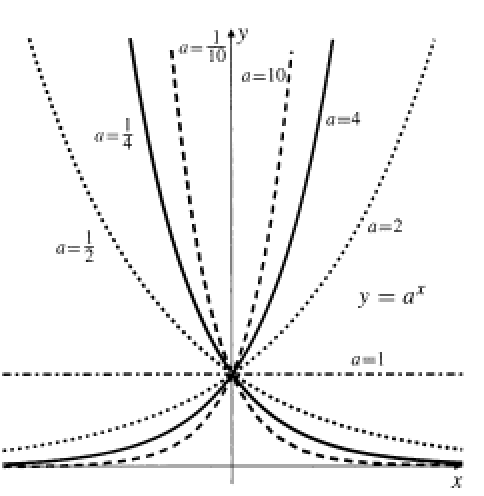
\includegraphics[scale=.6]{3-2-exponentials}
\end{figure}

\subsection*{Logarithm}

If $a >0$ and $a \neq 1$, the function $\log_a x$ called the \textbf{logarithm of $x$ base $a$} is the inverse of the 1-1 function $a^x$:
\[
    y = \log_a x \iff x = a^y
\]

Since $a^x$ has domain $(-\infty, \infty)$, and range $(0, \infty)$, $\log_a x$ has domain $(0, \infty)$ and range $(-\infty, \infty)$.

Since $a^x$ and $\log_a x$ are inverse functions
\[
    \log_a a^x = x \quad \forall x, \qquad a^{\log_a x} = x, \quad x>0
\]

\begin{figure}[H]
    \centering
    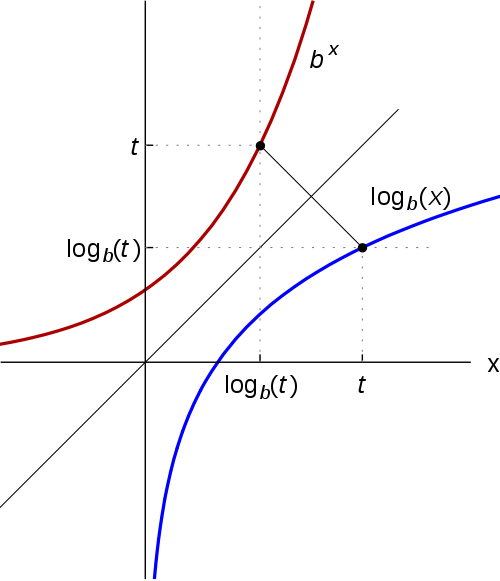
\includegraphics[scale=.3]{3-2-explog}
    \caption{The graph of logarithmic function is a reflection of the graph of the exponential function in the line $y = x$ (from Wikipedia).}
\end{figure}

\textbf{Laws of Logarithm}
If $x>0$, $y>0$, $a>0$, $b>0$, $a \neq 1$, $b \neq 1$, then

\begin{multicols}{2}
\begin{enumerate}
    \item $\log_a 1 = 0$
    \item $\log_a (x y) = \log_a x + \log_a y$
    \item $\log_a (\dfrac{1}{x}) = - \log_a x$
    \item $\log_a (\dfrac{x}{y}) = \log_a x - \log_a y$
    \item $\log_a x^y = y \log_a x$
    \item $\log_a x = \dfrac{\log_b x}{\log_b a}$
\end{enumerate}
\end{multicols}

\begin{example}
    Prove property $\log_a (x y) = \log_a x + \log_a y$ using laws of exponent.
\end{example}
\begin{solution}
    Take $u = \log_a x$, $v = \log_a y$ then $x = a^u$, $y = a^v$ and
    \[
        x y = a^{u+v} \iff u + v = \log(xy)
    \]
\end{solution}

\begin{example}
    Simplify
    \begin{enumerate}
        \item $\log_2 10 + \log_2 12 - \log_2 15$
        \[
            = \log_2 \frac{10 \times 12}{15} = \log_2 8 = 3
        \]
        \item $\log_{a^2} a^3$
        \[
             = \frac{\log_a a^3}{\log_a a^2} = \frac{3}{2}
        \]
        \item $3^{\log_9 4}$
        \[
             = 3^{\frac{1}{2} \log_3 4} = 3^{\log_3 2} = 2
        \]
    \end{enumerate}
\end{example}

\begin{example}
    Solve
    \[
        3^{x-1} = 2^x.
    \]
\end{example}
\begin{solution}
    \[
        (x-1) \log_{10} 3 = x \log_{10} 2 \iff
        x = \frac{\log_{10} 3}{\log_{10} 3/2}
    \]
\end{solution}
\end{document}